\documentclass[a4paper]{standalone}

\usepackage{amsmath,stmaryrd}
\usepackage{tikz}
\usepackage{mathdots}
\usepackage{yhmath}
\usepackage{cancel}
\usepackage{color}
\usepackage{siunitx}
\usepackage{array}
\usepackage{multirow}
\usepackage{amssymb}
\usepackage{gensymb}
\usepackage{tabularx}
\usepackage{booktabs}
\usetikzlibrary{fadings}

\usepackage[T1]{fontenc}
\usepackage[utf8]{inputenc}

\usepackage{pgfplots}

\begin{document}


$ $


\tikzset{every picture/.style={line width=0.75pt}} %set default line width to 0.75pt        

% This file was created by tikzplotlib v0.9.1.
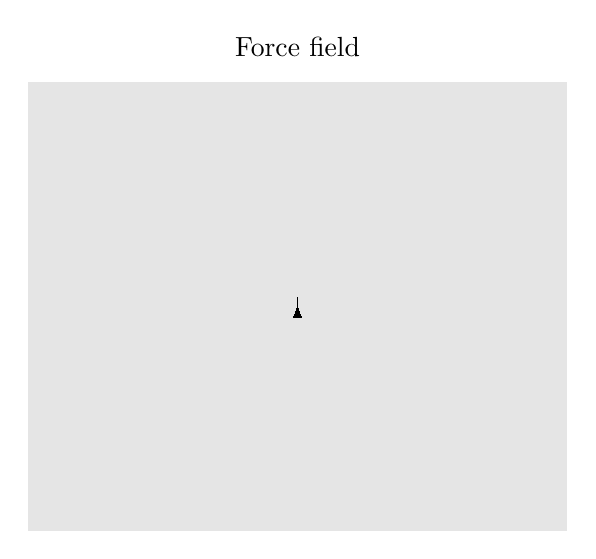
\begin{tikzpicture}

\begin{axis}[
axis background/.style={fill=white!89.8039215686275!black},
axis line style={white},
hide x axis,
hide y axis,
tick align=outside,
tick pos=left,
title={Force field},
x grid style={white},
xmajorgrids,
xmin=-0.5, xmax=0.5,
xtick style={color=white!33.3333333333333!black},
y dir=reverse,
y grid style={white},
ymajorgrids,
ymin=-0.5, ymax=0.5,
ytick style={color=white!33.3333333333333!black}
]
\draw[-latex,draw=black] (axis cs:0,0) -- (axis cs:0,0);
\draw[-latex,draw=black] (axis cs:0,0) -- (axis cs:0,0);
\draw[-latex,draw=black] (axis cs:0,0) -- (axis cs:0,0);
\draw[-latex,draw=black] (axis cs:0,0) -- (axis cs:0,0);
\draw[-latex,draw=black] (axis cs:0,0) -- (axis cs:0,0);
\draw[-latex,draw=black] (axis cs:0,0) -- (axis cs:0,0);
\draw[-latex,draw=black] (axis cs:0,0) -- (axis cs:0,0);
\draw[-latex,draw=black] (axis cs:0,0) -- (axis cs:0,0);
\draw[-latex,draw=black] (axis cs:0,0) -- (axis cs:0,0);
\draw[-latex,draw=black] (axis cs:0,0) -- (axis cs:0,0);
\draw[-latex,draw=black] (axis cs:0,0) -- (axis cs:0,0);
\draw[-latex,draw=black] (axis cs:0,0) -- (axis cs:0,0);
\draw[-latex,draw=black] (axis cs:0,0) -- (axis cs:0,0);
\draw[-latex,draw=black] (axis cs:0,0) -- (axis cs:0,0);
\draw[-latex,draw=black] (axis cs:0,0) -- (axis cs:0,0);
\draw[-latex,draw=black] (axis cs:0,0) -- (axis cs:0,0);
\draw[-latex,draw=black] (axis cs:0,0) -- (axis cs:0,0);
\draw[-latex,draw=black] (axis cs:0,0) -- (axis cs:0,0);
\draw[-latex,draw=black] (axis cs:0,0) -- (axis cs:0,0);
\draw[-latex,draw=black] (axis cs:0,0) -- (axis cs:0,0);
\draw[-latex,draw=black] (axis cs:0,0) -- (axis cs:0,0);
\draw[-latex,draw=black] (axis cs:0,0) -- (axis cs:0,0);
\draw[-latex,draw=black] (axis cs:0,0) -- (axis cs:0,0);
\draw[-latex,draw=black] (axis cs:0,0) -- (axis cs:0,0);
\draw[-latex,draw=black] (axis cs:0,0) -- (axis cs:0,0);
\draw[-latex,draw=black] (axis cs:0,0) -- (axis cs:0,0);
\draw[-latex,draw=black] (axis cs:0,0) -- (axis cs:0,0);
\draw[-latex,draw=black] (axis cs:0,0) -- (axis cs:0,0);
\draw[-latex,draw=black] (axis cs:0,0) -- (axis cs:0,0);
\draw[-latex,draw=black] (axis cs:0,0) -- (axis cs:0,0);
\draw[-latex,draw=black] (axis cs:0,0) -- (axis cs:0,0);
\draw[-latex,draw=black] (axis cs:0,0) -- (axis cs:0,0);
\draw[-latex,draw=black] (axis cs:0,0) -- (axis cs:0,0);
\draw[-latex,draw=black] (axis cs:0,0) -- (axis cs:0,0);
\draw[-latex,draw=black] (axis cs:0,0) -- (axis cs:0,0);
\draw[-latex,draw=black] (axis cs:0,0) -- (axis cs:0,0);
\draw[-latex,draw=black] (axis cs:0,0) -- (axis cs:0,0);
\draw[-latex,draw=black] (axis cs:0,0) -- (axis cs:0,0);
\draw[-latex,draw=black] (axis cs:0,0) -- (axis cs:0,0);
\draw[-latex,draw=black] (axis cs:0,0) -- (axis cs:0,0);
\draw[-latex,draw=black] (axis cs:0,0) -- (axis cs:0,0);
\draw[-latex,draw=black] (axis cs:0,0) -- (axis cs:0,0);
\draw[-latex,draw=black] (axis cs:0,0) -- (axis cs:0,0);
\draw[-latex,draw=black] (axis cs:0,0) -- (axis cs:0,0);
\draw[-latex,draw=black] (axis cs:0,0) -- (axis cs:0,0);
\draw[-latex,draw=black] (axis cs:0,0) -- (axis cs:0,0);
\draw[-latex,draw=black] (axis cs:0,0) -- (axis cs:0,0);
\draw[-latex,draw=black] (axis cs:0,0) -- (axis cs:0,0);
\draw[-latex,draw=black] (axis cs:0,0) -- (axis cs:0,0);
\draw[-latex,draw=black] (axis cs:0,0) -- (axis cs:0,0);
\draw[-latex,draw=black] (axis cs:0,0) -- (axis cs:0,0);
\draw[-latex,draw=black] (axis cs:0,0) -- (axis cs:0,0);
\draw[-latex,draw=black] (axis cs:0,0) -- (axis cs:0,0);
\draw[-latex,draw=black] (axis cs:0,0) -- (axis cs:0,0);
\draw[-latex,draw=black] (axis cs:0,0) -- (axis cs:0,0);
\draw[-latex,draw=black] (axis cs:0,0) -- (axis cs:0,0);
\draw[-latex,draw=black] (axis cs:0,0) -- (axis cs:0,0);
\draw[-latex,draw=black] (axis cs:0,0) -- (axis cs:0,0);
\draw[-latex,draw=black] (axis cs:0,0) -- (axis cs:0,0);
\draw[-latex,draw=black] (axis cs:0,0) -- (axis cs:0,0);
\draw[-latex,draw=black] (axis cs:0,0) -- (axis cs:0,0);
\draw[-latex,draw=black] (axis cs:0,0) -- (axis cs:0,0);
\draw[-latex,draw=black] (axis cs:0,0) -- (axis cs:0,0);
\draw[-latex,draw=black] (axis cs:0,0) -- (axis cs:0,0);
\draw[-latex,draw=black] (axis cs:0,0) -- (axis cs:0,0);
\draw[-latex,draw=black] (axis cs:0,0) -- (axis cs:0,0);
\draw[-latex,draw=black] (axis cs:0,0) -- (axis cs:0,0);
\draw[-latex,draw=black] (axis cs:0,0) -- (axis cs:0,0);
\draw[-latex,draw=black] (axis cs:0,0) -- (axis cs:0,0);
\draw[-latex,draw=black] (axis cs:0,0) -- (axis cs:0,0);
\draw[-latex,draw=black] (axis cs:0,0) -- (axis cs:0,0);
\draw[-latex,draw=black] (axis cs:0,0) -- (axis cs:0,0);
\draw[-latex,draw=black] (axis cs:0,0) -- (axis cs:0,0);
\draw[-latex,draw=black] (axis cs:0,0) -- (axis cs:0,0);
\draw[-latex,draw=black] (axis cs:0,0) -- (axis cs:0,0);
\draw[-latex,draw=black] (axis cs:0,0) -- (axis cs:0,0);
\draw[-latex,draw=black] (axis cs:0,0) -- (axis cs:0,0);
\draw[-latex,draw=black] (axis cs:0,0) -- (axis cs:0,0);
\draw[-latex,draw=black] (axis cs:0,0) -- (axis cs:0,0);
\draw[-latex,draw=black] (axis cs:0,0) -- (axis cs:0,0);
\draw[-latex,draw=black] (axis cs:0,0) -- (axis cs:0,0);
\draw[-latex,draw=black] (axis cs:0,0) -- (axis cs:0,0);
\draw[-latex,draw=black] (axis cs:0,0) -- (axis cs:0,0);
\draw[-latex,draw=black] (axis cs:0,0) -- (axis cs:0,0);
\draw[-latex,draw=black] (axis cs:0,0) -- (axis cs:0,0);
\draw[-latex,draw=black] (axis cs:0,0) -- (axis cs:0,0);
\draw[-latex,draw=black] (axis cs:0,0) -- (axis cs:0,0);
\draw[-latex,draw=black] (axis cs:0,0) -- (axis cs:0,0);
\draw[-latex,draw=black] (axis cs:0,0) -- (axis cs:0,0);
\draw[-latex,draw=black] (axis cs:0,0) -- (axis cs:0,0);
\draw[-latex,draw=black] (axis cs:0,0) -- (axis cs:0,0);
\draw[-latex,draw=black] (axis cs:0,0) -- (axis cs:0,0);
\draw[-latex,draw=black] (axis cs:0,0) -- (axis cs:0,0);
\draw[-latex,draw=black] (axis cs:0,0) -- (axis cs:0,0);
\draw[-latex,draw=black] (axis cs:0,0) -- (axis cs:0,0);
\draw[-latex,draw=black] (axis cs:0,0) -- (axis cs:0,0);
\draw[-latex,draw=black] (axis cs:0,0) -- (axis cs:0,0);
\draw[-latex,draw=black] (axis cs:0,0) -- (axis cs:0,0);
\draw[-latex,draw=black] (axis cs:0,0) -- (axis cs:0,0);
\draw[-latex,draw=black] (axis cs:0,0) -- (axis cs:0,0);
\draw[-latex,draw=black] (axis cs:0,0) -- (axis cs:0,0);
\draw[-latex,draw=black] (axis cs:0,0) -- (axis cs:0,0);
\draw[-latex,draw=black] (axis cs:0,0) -- (axis cs:0,0);
\draw[-latex,draw=black] (axis cs:0,0) -- (axis cs:0,0);
\draw[-latex,draw=black] (axis cs:0,0) -- (axis cs:0,0);
\draw[-latex,draw=black] (axis cs:0,0) -- (axis cs:0,0);
\draw[-latex,draw=black] (axis cs:0,0) -- (axis cs:0,0);
\draw[-latex,draw=black] (axis cs:0,0) -- (axis cs:0,0);
\draw[-latex,draw=black] (axis cs:0,0) -- (axis cs:0,0);
\draw[-latex,draw=black] (axis cs:0,0) -- (axis cs:0,0);
\draw[-latex,draw=black] (axis cs:0,0) -- (axis cs:0,0);
\draw[-latex,draw=black] (axis cs:0,0) -- (axis cs:0,0);
\draw[-latex,draw=black] (axis cs:0,0) -- (axis cs:0,0);
\draw[-latex,draw=black] (axis cs:0,0) -- (axis cs:0,0);
\draw[-latex,draw=black] (axis cs:0,0) -- (axis cs:0,0);
\draw[-latex,draw=black] (axis cs:0,0) -- (axis cs:0,0);
\draw[-latex,draw=black] (axis cs:0,0) -- (axis cs:0,0);
\draw[-latex,draw=black] (axis cs:0,0) -- (axis cs:0,0);
\draw[-latex,draw=black] (axis cs:0,0) -- (axis cs:0,0);
\draw[-latex,draw=black] (axis cs:0,0) -- (axis cs:0,0);
\draw[-latex,draw=black] (axis cs:0,0) -- (axis cs:0,0);
\draw[-latex,draw=black] (axis cs:0,0) -- (axis cs:0,0);
\draw[-latex,draw=black] (axis cs:0,0) -- (axis cs:0,0);
\draw[-latex,draw=black] (axis cs:0,0) -- (axis cs:0,0);
\draw[-latex,draw=black] (axis cs:0,0) -- (axis cs:0,0);
\end{axis}

\end{tikzpicture}


\end{document}